\documentclass[12pt]{article}
\usepackage[margin=2.0cm]{geometry}
\usepackage[utf8]{inputenc}
\usepackage[T1]{fontenc}
\usepackage[]{graphicx}
\usepackage{subfig}
\usepackage[]{braket}
\usepackage{setspace}%pacote para habilitar espaçamento duplo
\usepackage[english, brazilian]{babel}
\usepackage[]{float}%Pacote que permite fazer posicionamento específico de figura com parâmetro [H]
\usepackage[]{indentfirst}%primeiro parágrafo de cada seção começa a ter recuo
\usepackage[]{hyperref}%pacote para referência ao tipo também. comando \autoref
\usepackage[table,xcdraw]{xcolor}%Pacotes para geração de tabela
\usepackage{booktabs}%Pacotes para geração de tabela
\usepackage{caption}
\usepackage{subcaption}
\usepackage{booktabs}
\usepackage{biblatex}
\addbibresource{Bibliografia.bib}


%\usepackage{helvet} %Pacote para fonte Arial
%\renewcommand{\familydefault}{\sfdefault} %Pacote auxiliar para fonte arial.

%No site da CTAM há a documentação de cada um dos pacotes

\begin{document}

\begin{center}
    

{\bf UNIVERSIDADE FEDERAL DO ABC\\
CENTRO DE ENGENHARIA, MODELAGEM E CIÊNCIAS SOCIAIS APLICADAS }\\[0.7cm]

\begin{figure}[H]
    \centering
    
\includegraphics[scale=0.4]{Imagens/Ufabc_logo.png}
    \label{fig:ufabc_logo}
\end{figure}

{\large
    {\bf Trabalho de Graduação I}\\[0.7cm]
    {\bf Relatório}\\[0.7cm]
    {\bf Blockchain em meios de pagamento}
}\\[1.5cm]

Profº Dr. João Henrique Kleinschmidt\\[0.3cm]
Victor Hugo da Costa Leite                RA: 11039215\\[5.0cm]

Santo André\\Fevereiro de 2021
   
\end{center}
\newpage
\section{Introdução}

Blockchain nasceu em 2008 com a introdução do Bitcoin e na última década ganhou repercussão e importância a ponto de ser plataforma de diversas aplicações utilizada por empresas e governos. Blockchain é o nome da tecnologia de blocos encadeados que são compartilhados por nós em uma rede \emph{peer-to-peer} (P2P). Cada bloco da blockchain possui um conjunto de informações que depois que o bloco é construído e inserido na blockchain, as informações não podem ser alteradas e estarão replicadas e acessíveis por todos os nós da rede P2P.

Uma das aplicações blockchain mais famosas e mais utilizadas atualmente são as criptomoedas ou moedas digitais. Foi a primeira tecnologia que permitiu a existência de um ativo digital pois evita a replicação do ativo e seu gasto duplo que até antes do surgimento da tecnologia era impossível de ser evitado. A blockchain tem um processo de validação chamado de mecanismo de consenso onde a maioria dos nós da rede P2P precisam chegar a um consenso olhando nos registros dentro dos blocos da blockchain que o valor que está sendo gasto não está sendo gasto mais de uma vez.

Moedas físicas, geralmente estão sob o controle de uma entidade governamental podendo ter o seu valor alterado com a impressão de dinheiro e também necessitam de entidades intermediárias que cobram taxas para realização de transações financeiras o que de certa forma diminui a liberdade da movimentação de dinheiro e impõe limites devido aos custo operacionais de se fazer movimentações financeiras. Moedas digitais tem como característica, trazida pela blockchain funcionar em cima de uma rede P2P e possuir o mecanismo de consenso, a sua descentralização. Transações financeiras com moedas digitais podem ser executadas sem entidades de confiança e que cobram taxas, como bancos e o banco central, pois o mecanismo de consenso irá validar e impedir ações maliciosas.

Apesar da existência de moedas digitais com valor financeiro, hoje em dia moedas digitais não são amplamente utilizadas como meio de pagamento. Uma transação financeira utilizando moeda digital é demorada pois precisa esperar o mecanismo de consenso agir numa escala global, não está livre de custo pois a inserção de uma transação na blockchain precisa remunerar os mineradores e não é escalável uma vez que as blockchains mais usadas e conhecidas conseguem processar cerca de 30 transações por segundo, o que é muito menor do que a média de processamento da Visa de 1700 transações por segundo. Como uma solução para essas questões inerentes a tecnologia de blockchain foi criada uma segunda camada em cima da blockchain, o que faz a solução final ter os mesmos benefícios que a blockchain tem, chamada de Payment Channel Network (PCN). O PCN faz não ser mais necessário que toda transação financeira precise entrar na blockchain imediatamente fazendo com que um pagamento seja quase instantâneo, escalável e sem custo. O único custo envolvido é o de abrir e fechar um canal de pagamento com um remetente que precisa ser feito por meio de processo transacional na blockchain.

Tendo uma tecnologia que permita pagamentos rápidos e sem custo independente do valor, torna viável um conceito não novo que é o conceito de micropagamentos. Um micropagamento é definido como um pagamento de baixo valor financeiro. Micropagamentos até então tinham o problema que o valor do pagamento era muitas vezes muito próximo ou menor do que o valor das taxas envolvidas cobradas por entidades bancárias como um custo operacional. A viabilidade de micropagamentos torna possível uma nova modalidade de consumir produtos e serviços que até então não podiam ser consumidos sob demanda.

Este relatório aborda os temas estudados como blockchain, criptomoedas e PCN que possibilitarão a construção de uma aplicação cujo consumo de conteúdo possa ser feito sob demanda através do pagamento de valores pequenos, impraticáveis com modelos de pagamentos existentes no mercado hoje.

\section{Fundamentação Teórica}

\subsection{Blockchain}

Blockchain é uma tecnologia emergente que se baseia no uso de uma estrutura de dados distribuída entre nós de uma rede \emph{peer-to-peer} (P2P) para a criação e armazenamento de transações feitas entre usuários da aplicação blockchain. Cada nó possui a mesma lista de blocos da blockchain em que cada bloco possui um conjunto de transações. Os nós, com devido poder para, podem inserir e validar novos blocos na blockchain sem nunca poderem remover ou alterar blocos já existentes o que garante um histórico íntegro e acessível de dados em todos os nós.

Os nós da blockchain são encarregados de fazerem a criação e validação de novos blocos por meio de técnicas de consenso que garantem uma consistência e sincronização eventual dos dados da blockchain ao longo do tempo. É o mecanismo de consenso que permite que nós não mutuamente confiáveis cheguem a um comum acordo dado que a maioria dos nós concordem~\cite{braga2017segurancca}.

\subsection{Estrutura de dados}

A estrutura de dados do blockchain, como o nome sugestivamente diz, é uma lista ligada de blocos em que o bloco mais recente aponta para o bloco anterior e assim sucessivamente até o primeiro bloco da blockchain que é chamado de \emph{genesis}.

Cada bloco da blockchain é constituído por um cabeçalho e por um conjunto de transações. Um cabeçalho simplificado de um bloco possui informações como: o \emph{hash} do bloco anterior, um número pseudoaleatório \emph{nonce}, o hash do bloco inteiro e o \emph{hash} da raiz da árvore de Merkle que é a estrutura de dados na qual o conjunto de transações está organizado.

Como já dito, o conjunto de transações é organizado em um árvore de Merkle onde as folhas da árvore são as transações propriamente ditas. O segundo nível da árvore é composto pelo hash de cada uma das transações e os demais níveis são os hash de pares de hash dos níveis anteriores até que se chegue na raiz da árvores, cujo hash é armazenado no cabeçalho do bloco. A figura \ref{fig:estrutura_blockchain} mostra uma representação de um bloco da blockchain.

\begin{figure}[H]
    \centering
    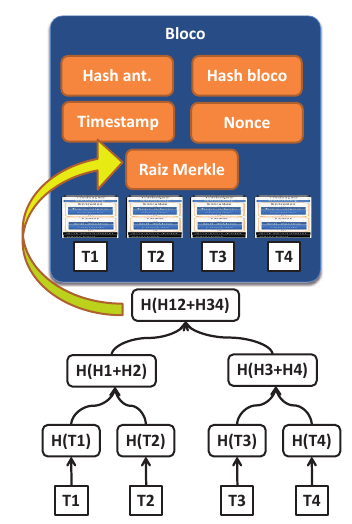
\includegraphics[scale=0.4]{Imagens/estrutura_blockchain.png}
    \caption{Estrutura de um bloco da blockchain.}
    \label{fig:estrutura_blockchain}
\end{figure}

Uma função \emph{hash} possui a propriedade de \textbf{resistência à colisão} em que idealmente é impossível encontrar dois \emph{hashs} iguais de tal forma que $H(a) = H(b)$ onde $a$ e $b$ são mensagens diferentes e propriedade de \textbf{ocultação} em que dado $H(a)$ é inviável encontrar $a$. O uso de funções hash na árvore de Merkle das folhas até a sua raiz faz com que possamos conferir a integridade das transações presentes no bloco, isto é, conferir de não houve alteração na transação depois de inserida no bloco. Para isso basta ir calculando o hash das folhas até o hash da raiz e comparar com o hash presente no cabeçalho do bloco. Para certificar que as transações estão íntegras basta que o hash resultante da raiz seja igual ao hash presente no cabeçalho.

Além disso, também é calculado o hash do bloco utilizando todos os dados do cabeçalho. Como o bloco seguinte conterá o hash do bloco atual, para verificar a integridade do bloco como um todo basta comparar o hash do bloco atual contido no bloco seguinte com o hash calculado do bloco atual. Assim, com os cálculos de hash de um bloco feito em $O(log(n))$ pode-se verificar a integridade de um bloco e de toda uma cadeia de blocos.

O conjunto de transações armazenadas em uma blockchain, também chamadas de livro razão~\cite{greve2018blockchain}, são texto livre onde a semântica vai de acordo com as necessidades da aplicação que está sendo construída. No caso de uma aplicação de pagamentos muito provável que o conjunto de transações se pareça com um livro contábil que contém dados de onde está saindo o dinheiro, quanto está saindo e para quem está indo o dinheiro, além de uma assinatura digital sobre o hash da transação feito pela pessoa que está transferindo. Tal assinatura confere a autorização e autenticidade da pessoa que está transferindo. Geralmente as assinaturas são feitas utilizando assinaturas de chave pública e chave privada o que torna possível o requisitante da transação assinar uma transação e outros validarem a assinatura utilizando a chave pública. A blockchain somente garante que os dados inseridos na blockchain não podem ser alterados ou trocados de ordem. Quaisquer outras validações sobre os dados que sejam mais específicas devem ser de responsabilidade da camada de aplicação. 

No caso de uma aplicação financeira, uma última etapa de validação ocorre verificando se a mesma transação com os mesmos valores referenciados já não foi utilizada, o que implicaria em duplo gasto. Para isso é necessário efetuar uma busca na blockchain começando no bloco da transação referenciada até o último bloco da estrutura.

Outros campos que podem estar presentes nos blocos de uma blockchain são um campo de timestamp do momento que o bloco é criado, um valor arbitrário chamado \textit{nonce} que tem o objetivo de dar variabilidade para o hash calculado do bloco e metadados em geral que podem conter a chave pública de quem fez a \emph{mineração} do bloco e outras informações que dependem da blockchain\cite{miers2019analise}.

\subsection{Propriedades}

A tecnologia blockchain permite que aplicações construídas em cima dela tenham algumas propriedades intrínsecas:
\begin{itemize}
    \item Descentralização: Todos os nós da rede P2P possuem uma cópia da base de dados distribuída e dependendo do modelo de blockchain todos os nós conseguem validar transações feitas entre nós, não confiáveis entre si, sem a necessidade de uma terceira entidade confiável.
    \item Disponibilidade: Como a base de dados de transações é distribuídas entre todos os nós da rede e a criação de blocos também consegue ser feita por todos os nós da rede sem a dependência de uma entidade única, caso alguns nós fiquem indisponíveis por algum motivo o restante da rede ainda consegue fazer todo o trabalho necessário para que a blockchain não pare de funcionar.
    \item Integridade: Todas as transações são assinadas com a chave privada do autor e validada posteriormente por outros nós da rede P2P fazendo com que todas as transações inseridas no blockchain sejam integras. Além disso, existem a noção de ordem de criação de transações graças a verificação de hash do bloco anterior o que permite validar a ordem geral das transações também.
    \item Auditabilidade: Como uma vez inserido o bloco em um blockchain ele não pode ser alterado ou removido e toda a base de dados está replicada nos diversos nós da rede P2P, é garantida alta auditabilidade na blockchain.
    \item Imutabilidade e Irrefutabilidade: A estrutura de dados da blockchain faz com que se um bloco seja alterado uma validação da blockchain apontaria que ela está inválida. Além disso, como as transações são assinadas, somente é possível fazer alterações na blockchain por meio da inserção de novas transações e novos blocos.
\end{itemize}

\subsection{Mecanismo de Consenso}

A inserção de um bloco na blockchain consiste em criar o bloco e distribuí-lo para outros nós da blockchain. Uma vez recebido um bloco, ele é verificado e, se estiver válido, repassado para os demais blocos da blockhain até que todos os nós tenham um cópia do bloco. A consistência do livro-razão é alcançada no momento em que "todos os usuários tenham a mesma visão sobre a ordem em que os blocos foram inseridos na cadeia"\cite{miers2019analise}.

Devido o processo de propagação do bloco nos nós de uma blockchain ser assíncrono e sem uma coordenação central, então exige-se um mecanismo de consenso que garanta a convergência da visão que cada nó tem sobre o estado da blockchain em um espaço de tempo não muito longo. Esse mecanismo de consenso tem o objetivo de garantir que a blockchain permaneça consistente ao que diz respeito à ordenação de blocos e sobre integridade do seu conteúdo. O mecanismo de consenso é posto em prática por vários nós não mutuamente confiáveis e por isso é o que garante a segurança e confiabilidade da rede.

\subsubsection{Comunicação e troca de mensagens}

Como a blockchain é um sistema distribuído, a troca de mensagens para propagar blocos está associado com mecanismo de distribuição de mensagens em que não há uma coordenação central e cada nó deve transmitir informação para outros nós que se sabe que estão participando do sistema. Geralmente cada nó possui uma lista, não necessariamente completa, de outros nós onde informações são transmitidas para por meio de protocolos de broadcasting\cite{miers2019analise}.

Muitas blockchains adotam a estratégia de existir nós que tem uma lista de todos os participantes da rede, assim na conexão de um novo nó são escolhidos nós aleatórios para que sejam passados para o novo nó e esse novo nó possa fazer o broadcasting.

\subsubsection{Regras de consenso}

No mecanismo de consenso deve existir um conjunto de regras que visam permitir que cada nó independente do sistema possa aplicar para validar transações, resolver conflitos e lidar com \emph{falhas bizantinas}. \emph{Falhas Bizantinas} são "falhas que podem apresentar-se de forma diferente para observadores distintos, devido à ausência de uma visão global da rede, criando então inconsistências no sistema"~\cite{miers2019analise}.

As regas de consenso podem resultar em dois tipos de consenso diferente: determinístico e probabilístico. No consenso determinístico, uma vez alcançado o consenso, a informação armazenada na blockchain não pode ser alterada posteriormente. No consenso probabilístico, um consenso posterior pode ir contra um consenso feito em um momento de tempo passado. Um exemplo de consenso probabilístico é o de em blockchains que aplicam a regra de armazenar localmente a versão da blockchain que apresente o maior número de blocos.

Na blockchain vários nós estão fazendo a mesma coisa e portanto há um dinamismo intrínseco ao processo de criação e inserção de blocos na blockchain onde todos os nós estão competindo para fazer a montagem de blocos e validação das transações visíveis a cada nó antes dos concorrentes. Uma vez que um bloco consegue fazer uma validação pelo processo de consenso da blockchain toda a rede precisa ser informada para que o bloco seja armazenado na cadeia de blocos~\cite{braga2017segurancca}.

Ao final da construção e validação de um novo bloco, os algorítimos de consenso pagam uma recompensa ao minerador pelo esforço computacional. Essa recompensa é feito pois "a segurança dos protocolos de consenso em blockchain é baseada na suposição de que a maioria dos operadores dos nós da rede P2P (os mineradores) está mais interessada em se beneficiar dos mecanismos de incentivo do protocolo e menos propensa a quebrar as regras"~\cite{braga2017segurancca}.

\subsubsection{Algoritmos de inserção de blocos}

Para atingir uma consistência na blockchain, a inserção de blocos não pode ser feita por todo e qualquer nó pois se fosse dificilmente chegaria o momento em que todos os nós da rede teriam a mesma visão do estado da blockchain. Portanto, deve existir um mecanismo de inserção de blocos que aumente a convergência do estado do sistema. A seguir estão alguns dos principais:
\begin{itemize}
    \item Prove of Work(PoW): Neste processo de inserção todos os nós da rede podem competir para validar transações e inserir novos blocos. Os nós que querem fazer o processo de validação e inserção são chamadas de mineradores e devem realizar uma tarefa primeiro para que ganhem o direito de validar e inserir. A tarefa no processo de PoW é o de "encontrar uma entrada cujo valor de hash seja menor que um determinado alvo"~\cite{miers2019analise}. Fazer a mineração é um processo altamente custoso computacionalmente e portanto uma desvantagem deste método é o tempo que leva para ser completada a mineração e o custo energético associado. Atualmente é o método utilizado pelo Bitcoin e Ethereum
    
    \item Prove of Stake(PoS): No PoS apenas nós que possam oferecer garantias, em termos de tokens, podem participar. Nesse processo, validadores são escolhidos aleatoriamente para criar blocos e para validar blocos que eles não criaram. A garantia é para que o nó sofra penalidades com perdas financeiras caso haja alguma anomalia na criação ou validação de blocos ou seja percebido algum comportamento malicioso por parte do nó. Deste modo espera-se que as consequências de um mau comportamento sejam mais caros do que agir corretamente. A blockchain de Ethereum está lançando um nova versão que migrará do atual uso de PoW para PoS. Por não ter a mineração feita no PoW espera-se ganhar em termos de economia energética e tempo com a atualização.   
\end{itemize}

\subsection{Modelos Blockchain}

As blockchains de hoje em dia podem ser classificadas em respeito ao seu acesso em:

    \subsubsection{Pública}Modelo que pode ser considerado completamente descentralizada. Qualquer nó pode participar do processo de consenso distribuído, ler e enviar transações.
    \subsubsection{Privada}Modelo completamente centralizado no qual uma instituição possui o total controle sobre as operações.
    \subsubsection{Consórcio}Modelo híbrido parcialmente centralizado em que duas ou mais instituições possuem o controle sobre as operações.
    

\subsection{Fluxo de inserção de blocos}
De acordo com \cite{braga2017segurancca} o fluxo resumido de inserção de blocos em uma blockchain pode ser resumido nos seguintes passos:
\begin{enumerate}
    \item Alice e Bob criam uma conta cada na blockchain.
    \item Alice divulga o endereço da sua conta para Bob.
    \item Bob forma uma transação e a assina digitalmente para o endereço de Alice;
    \item Bob propaga a transação propaga a transação entre os nós da rede P2P via um nó da rede.
    \item A transação é incluída em um bloco e os nós da rede trabalham para obter um consenso sobre a criação do bloco de acordo com o menismo de consenso empregado na blockchain.
    \item Os nós da rede P2P propagam o seu resultado para outros nós.
    \item Alice consulta o livro razão e entende que a sua transação foi aceita.
\end{enumerate}
Os passos descritos acima podem ser visualizados na figura \ref{fig:transacao_blockchain}. Um ponto importante de frisar aqui é que do momento que a transação é submetida para validação na blockchain até o momento que ela pode ser consultada há o delay do funcionamento do mecanismo de consenso e propagação de blocos por toda a rede P2P. Assim, no momento que estiver sendo criada uma aplicação em cima de uma blockchain esse delay deve ser levado em conta já que é intrínseco aos mecanismos de consenso utilizados hoje em dia.
\begin{figure}[H]
    \centering
    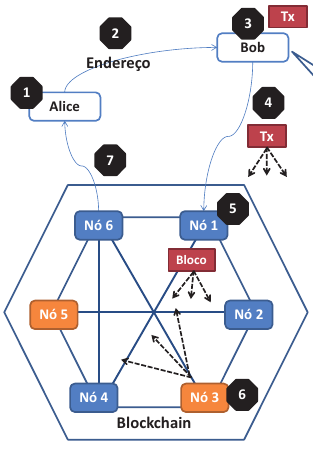
\includegraphics[scale=0.7]{Imagens/passos_transação.png}
    \caption{Fluxo de transação na blockchain.}
    \label{fig:transacao_blockchain}
\end{figure}

\subsection{Contratos Inteligentes}

Como já dito, as transações de uma blockchain são texto livre e seu conteúdo depende da semântica da aplicação. A partir dessa liberdade no uso de blockchain foi criado o conceito de contratos inteligentes. Contratos inteligentes são "programas de computador seguros e imparáveis que representam acordos executáveis e exigíveis automaticamente"~\cite{braga2017segurancca}. Estes programas são implantados como transações na blockchain. Eles rodam nos nós da rede de blockchain e funcionam automaticamente em benefício dos participantes da rede. 

Quando implantado o binário do contrato para a blockchain ele não pode mais ser impedido de rodar uma vez que a condições programadas sejam atingidas e portanto o que foi programado é o que será executado em todos os nós da rede P2P. Essa característica de inviolabilidade de código é interessante para execução de acordos em que não existem necessariamente confiança entre duas ou mais parte envolvidas. Com o uso de contratos inteligente, uma vez feito um acordo e implantado na blockchain ele será executado nas condições previstas sem qualquer entidade confiável controlando o processo.

\subsection{Aplicativos Descentralizados}

Uma vez que foi explicado como é o funcionamento de uma blockchain e que as transações podem possuir um aspecto geral em que contratos inteligentes podem ser utilizados de diversas formas, uma blockchain pode ser usada como infraestrutura para a criação do que chamamos de Decentralized Applications ou DApps. Os DApps possuem todas as propriedades discutidas pois os dados transacionais dos usuários estarão armazenados na blockchain e para as atividades executadas no aplicativo deverão ser submetidos novas transações para o mecanismo de consenso da blockchain. Exemplos de DApps são produtos de transações financeiras, cartórios, eleições, doações e vários outros onde a confiabilidade, imutabilidade, autenticidade, e integridade podem ser úteis.

Um DApp pode ser construído com uma arquitetura pensando nos seguintes componentes \cite{braga2017segurancca}:

\begin{enumerate}
    \item Frontend: camada que os usuários usarão para interagir com a aplicação. Normalmente é um aplicativo para smartphone e/ou um website que mandarão requisições para um backend.
    \item Aplicação servidora: backend cujo o frontend trocará mensagens com. É a camada responsável por conter regras de negócios do produto e poderá ter um banco de dados próprio além de ser responsável de criar transações para a blockchain.
    \item Integração aplicação com blockchain: interface de programação de aplicações (Application programming
Interface - API) responsável por servir de ponte entre o backend da aplicação servidores com a blockchain.
    \item Aplicação Blockchain: Aplicação responsável por manipular o livro razão através de um API.
    \item Contratos inteligente: Contrato que está presente em cada um dos nós da rede P2P e é responsável por implementar transações de semântica complexa na plataforma blockchain. 
\end{enumerate}

A figura \ref{fig:aplicacao_blockchain} mostra os componentes descritos acima na arquitetura de uma aplicação blockchain.

\begin{figure}[H]
    \centering
    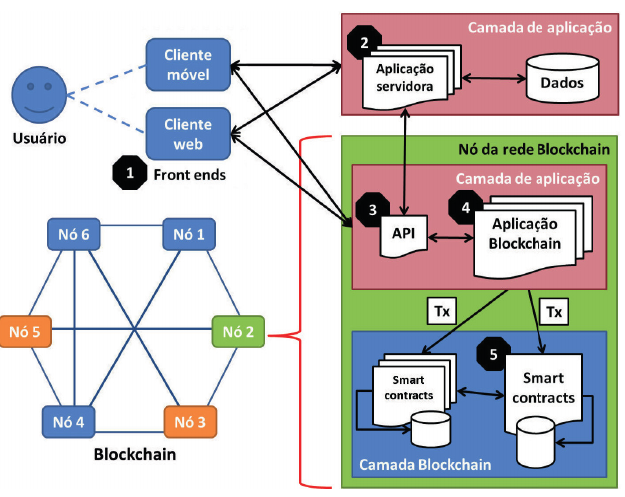
\includegraphics[scale=0.7]{Imagens/estrutura_dapp.png}
    \caption{Estrutura de uma aplicação blockchain.}
    \label{fig:aplicacao_blockchain}
\end{figure}

\section{Aplicações Financeiras}
\subsection{Moedas Digitais}

O conceito de blockchain foi introduzido na apresentação de uma aplicação específica que foi a criação da primeira moeda digital descentralizada. As propriedades de uma blockchain, permitiram a criação do Bitcoin introduzido em \cite{nakamoto2008peer} em 2008. Como imaginado, esta moeda digital não teria a entidade de um banco central controlando ela e podendo alterar o seu valor a partir da impressão de uma moeda. Hoje o único jeito de se criar um bitcoin é através do processo de mineração do mecanismo de consenso PoW sendo que nesse processo foi previsto no código do bitcoin a limitação da quantidade de moedas produzidas ao longo do tempo e está previsto que limite o número máximo de bitcoins que poderão ser gerados.

Desde a criação do bitcoin muitas outras moedas digitais surgiram e muitas delas possuem valor financeiro real o que permite que as moedas digitais possam ser usadas como meios de pagamento. 

\subsection{Micropagamentos}

Micropagamentos são transações financeiras cujo valor financeiro é muito pequeno e que geralmente são feitas de maneira online. Um grande empecilho para a adoção de micropagamentos é que muitas vezes as taxas das transações financeiras cobradas por entidades que intermedeiam o pagamento excedem o valor que se quer transferir. Desse modo, por não existirem essas entidades nas transferências de moedas digitais elas são um grande candidato para servir como meio de pagamento para micropagamentos

\subsection{Limitações da blockchain em pagamentos}

Apesar de moedas digitais em cima de blockchain não terem entidades intermediadoras entre transferências, pagamento com moedas digitais ainda possuem certas limitações \cite{mercan2021cryptocurrency}.
\begin{enumerate}
    \item Escalabilidade - A blockchain do bitcoin consegue lidar com certa de 7 transações por segundo e a blockchain Ethereum com Ether consegue lidar com cerca de 30 transações por segundo. Números bem abaixo do que a Visa consegue fazer hoje de cerca 1700 transações por segundo.
    \item Taxa de transações - apesar de não ter entidades intermediadores como bancos, a submissão de uma transação para a Ethereum, por exemplo, tem um custo associado impactando no custo final do micropagamento. 
    \item Tempo de confirmação - como já discutido, a submissão de uma transação para inserção na blockchain tem o delay do processo consenso e distribuição do novo bloco pela rede atrelado. Este tempo de espera faz com que um pagamento seja um processo demorado quando deveria ser quase instantâneo. 
\end{enumerate}

Apesar de blockchains terem permitido a existência de um ativo digital com valor financeiro mesmo sem uma entidade confiável como um banco central e bancos intermediários, as limitações acima dificultam o uso de moedas digitais como soluções de pagamentos. 

\subsection{Payment Channel Network (PCN)}

PCN é uma estratégia de realizar transações fora da cadeia (off-chain) da blockchain até que em algum momento elas sejam executadas todas de uma vez na blockchain (on-chain) passando pelo processo de consenso\cite{mercan2021cryptocurrency}. No método PCN contratos inteligentes são utilizados para uma conta $A$ transferir para outra conta $B$ onde o contrato assinado por $A$ serve como um cheque que $B$ pode usar para recuperar o valor de forma on-chain. Para esse método basta assinar um contrato para realizar um pagamento e enviá-lo por meio de um canal então o tempo de latência é ínfimo comparado ao do processo que precisa de consenso. Além disso como a comunicação ocorre no canal entre $A$ e $B$, podendo existir canais intermediários, então não há problemas de escalabilidade como o presente em um pagamento on-chain. E por fim, como será visto, a única taxa existente é na abertura de um canal entre duas contas então os pagamentos podem ser feitos praticamente sem taxas retirando todos os problema encontrados em uma blockchain para a realização de micropagamentos.

A ideia básica de se fazer transações off-chain é de evitar o processo de consenso para toda e qualquer pagamento. O PCN é uma camada que funciona em cima da blockchain. Toda o funcionamento é feito em volta de Canais de Pagamento~\cite{raidenmedium}. Um Canal de pagamento pode ser aberto entre duas contas quaisquer. A abertura de um canal de pagamento ocorre quando o remetente reserva um certo valor on-chain que ficará disponível em um contrato inteligente para que, mediante a apresentação de uma assinatura do remetente, o destinatário possa "sacar" o valor posteriormente. O valor reservado no contrato nunca pode ser maior do que o valor que o remetente tem disponível on-chain e uma vez o valor estando no contrato não pode ser usado para outra coisa que não para o destinatário realizar o saque.

Importante notar que na abertura de um canal um contrato está tendo o seu estado modificado e portanto tem um custo transacional da blockchain envolvido assim como precisa ter a transação validada pelo consenso. Da mesma forma, no "saque" de token ocorre a modificação do estado de um contrato e portanto também tem um custo transacional envolvido e precisa aguardar o processo de consenso.

Apesar do processo de abertura de canal entre um remetente $A$ e um destinatário $B$ ter um custo associado, não é necessário a abertura de um canal com toda e qualquer conta que se deseja fazer um pagamento devido a possibilidade de uso de uma rede de canais de pagamento que é criada entre as contas. Se uma conta $A$ quer realizar um pagamento para uma conta $C$ e ambas possuem um canal aberto com $B$ cujo valor depositado nos canais seja menor do que o valor do pagamento então é possível realizar o pagamento entre $A$ e $C$ com intermédio de $B$ off-chain. Um pagamento pode ser realizado por meio de quantos canais necessário desde que todos possuam um valor maior do que o valor do pagamento.

\section{Metodologia}
     
\subsection{Ethereum}

A Ethereum é uma blockchain de propósito geral que oferece a possibilidade de rodar contratos inteligentes através de uma camada de abstração Ethereum Virtual Machine (EVM) que conecta o client da máquina local com o restante da rede usando uma criptomoeda própria denominada \textit{Ether}. A Ethereum é uma blockchain pública e portanto qualquer pessoa pode criar e ler transações e participar do processo de consenso PoW na versão antiga e PoS na versão nova. Por ser pública também tem uma composição da rede desconhecida com a entrada e saída aleatória de nós. 

O contrato da Ethereum possui uma linguagem própria de escrita que é o Solidity. Cada operação realizada por um contrato está associado a um custo de execução de \emph{gas} que é o "combustível" consumido na operação\cite{miers2019analise}. 
O Ethereum possui sua própria forma para financiar a validação de blocos e monetizar a mesma, o seu "combustível", como é definido pela plataforma, é conhecido como Ether. O Gas é uma forma de desacoplar o custo das transações no Ethereum do câmbio flutuante da criptomoeda Ether, estabelecendo um custo para cada trabalho computacional.

O aspecto de propósito geral da linguagem solidity empregada nos contratos inteligentes faz com que da Ethereum possam nascer aplicações diversas, não necessariamente financeiras, que utilizem a infraestrutura da blockchain já existente sem a necessidade de criar uma blockchain nova. Ethereum é uma das plataformas mais utilizadas em projetos pilotos atualmente e também uma das tecnologias blockchain mais estudadas. Existem ambientes de desenvolvimento (IDEs), como o Browser Solidity e o Ethereum Studio.

\begin{figure}[H]
    \centering
    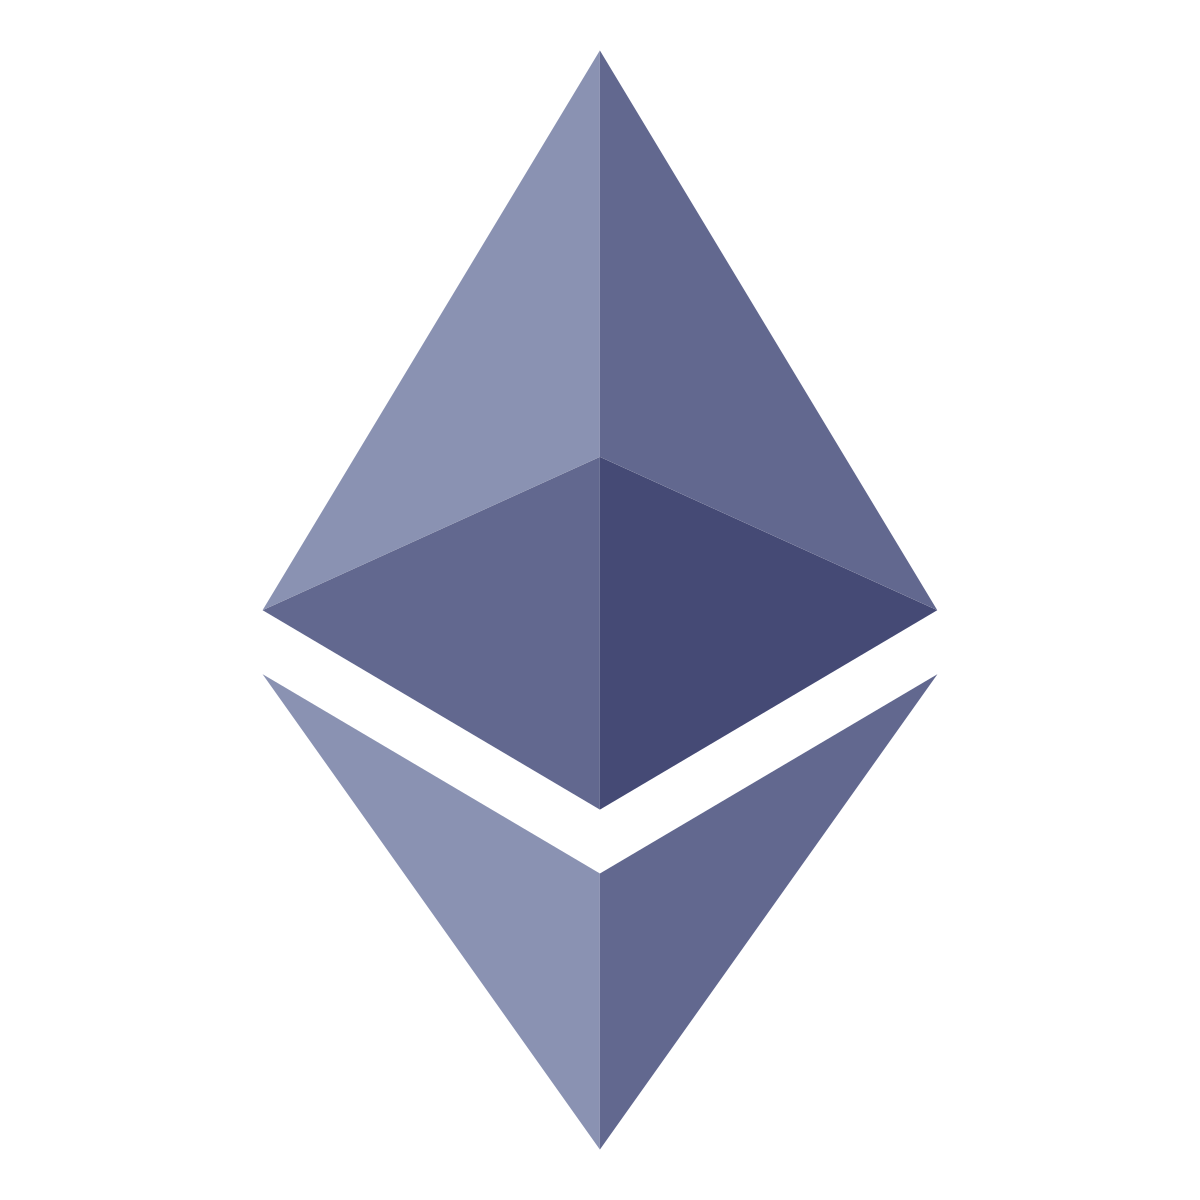
\includegraphics[scale=0.1]{Imagens/ethereum.png}
    \caption{Símbolo Ethereum.}
    \label{fig:ethereum_simbol}
\end{figure}

\subsection{Raiden}
     
 Raiden Network é uma solução Off-chain que implementa em cima do blockchain Ethereum o conceito de PCN. A implementação de uma PCN é complexa e não trivial o que dificulta o processo de desenvolvimento de aplicações de pagamento com moedas digitais. Apesar disso, toda a complexidade de implementação do PCN é abstraída através de uma API de fácil uso o que permite um desenvolvimento de soluções descentralizadas e escaláveis de maneira mais fácil. Raiden Network é compatível com o pagamento de qualquer token ERC20~\cite{raidenmedium}.
     
\begin{figure}[H]
    \centering
    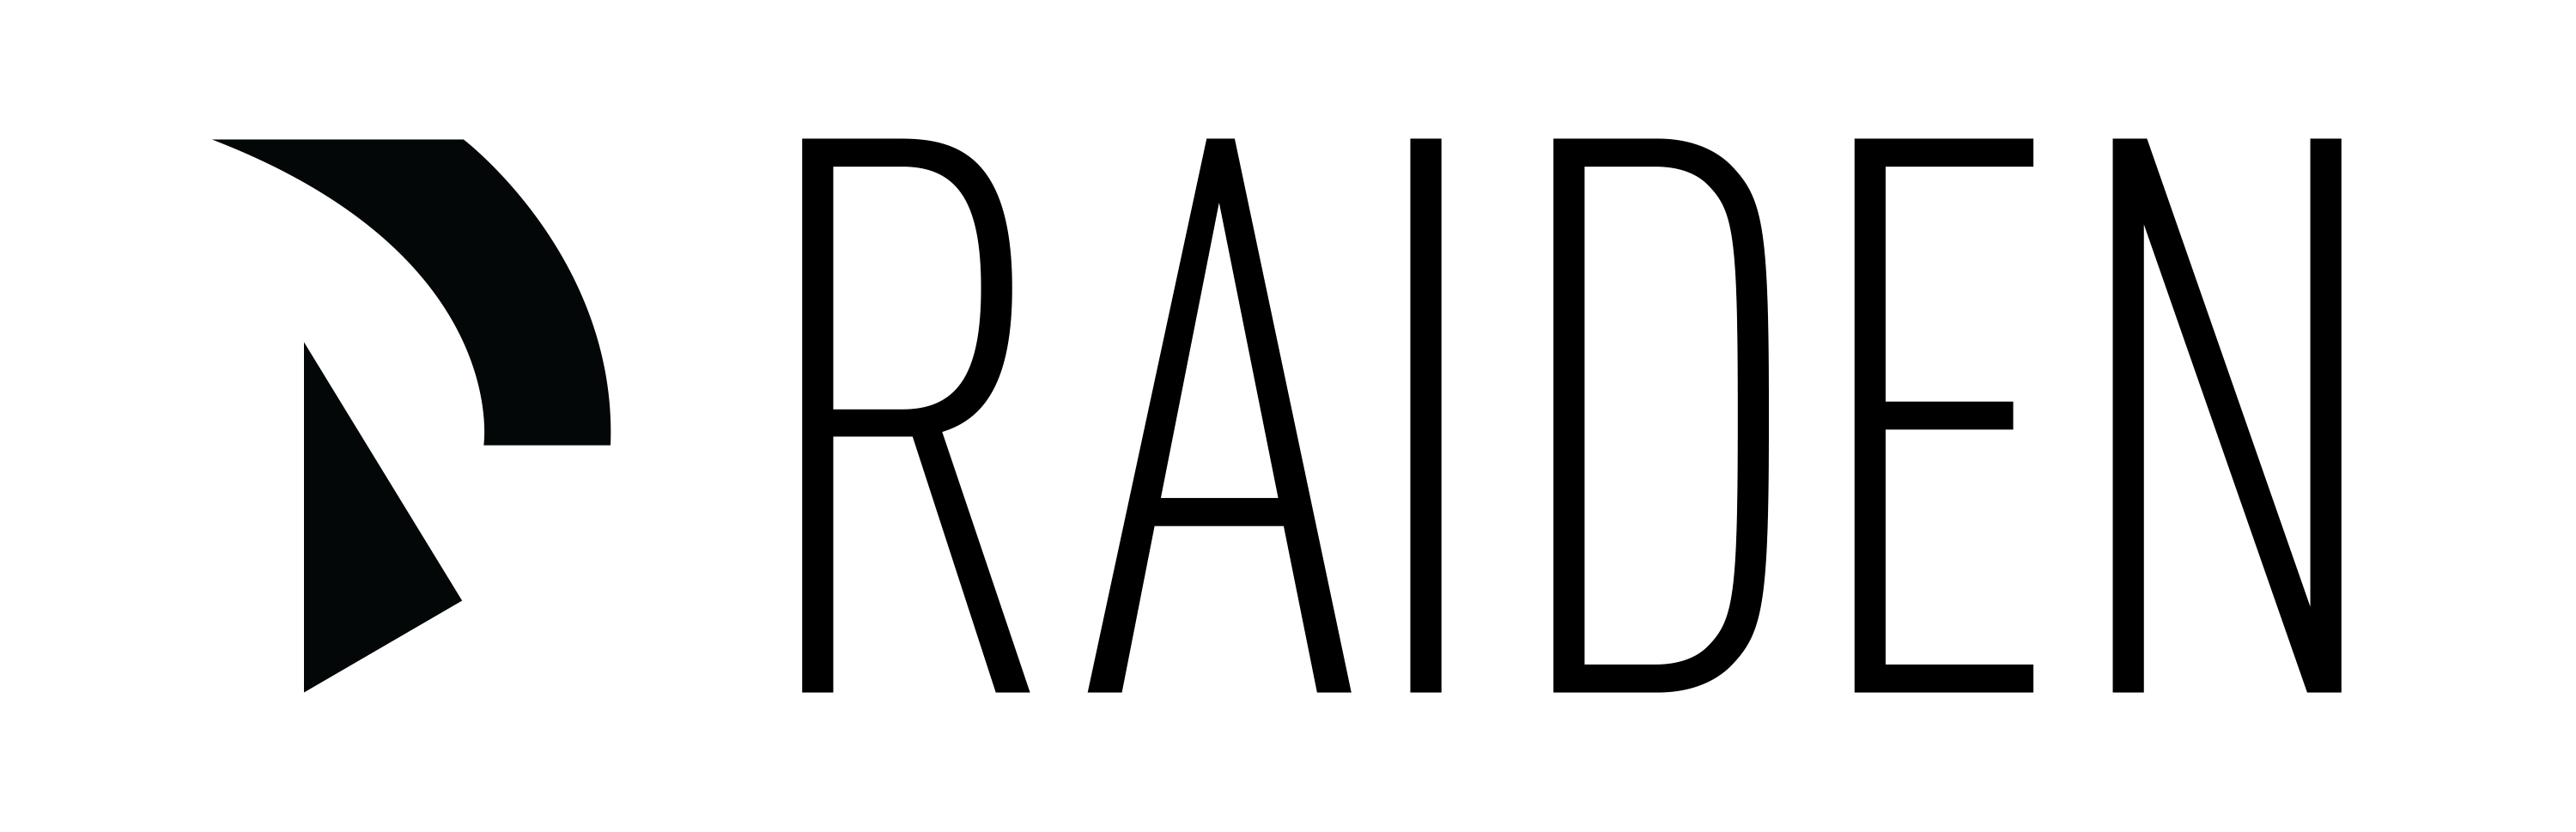
\includegraphics[scale=0.4]{Imagens/raiden.png}
    \caption{Símbolo Raiden.}
    \label{fig:raiden_simbol}
\end{figure}

\subsection{Aplicação}

Neste trabalho de graduação será feito o uso dos conceitos estudados utilizando a blockchain Ethereum e o framework Raiden para a construção de uma aplicação que permita fazer o uso de micropagamentos para consumo de determinado produto. Diversas provas de conceito utilizando blockchain nascem usando Ethereum pois é uma plataforma de propósito geral com ampla documentação na internet, cursos e casos de uso e por isso ela foi escolhida para este trabalho. Como o foco do TG é o uso de blockchain para micropagamentos a solução final precisará usar o Raiden que funciona em cima da Ethereum para sobrepor as limitações de escalabilidade, custo e tempo de espera de processamento. 

A aplicação construída deverá liberar o consumo de conteúdo como artigos jornalísticos, vídeos, músicas ou consumo de serviços de streaming por demanda sendo que a sua disponibilização do conteúdo ocorrerá mediante um pagamento de pequeno valor, configurando um micropagamento.

\singlespacing
\newpage
\printbibliography
\end{document}